\begin{frame}
\frametitle{Définitions Fondamentales des Graphes}

\begin{tcolorbox}[colback=orange!10,colframe=orange!100!black,
    title=Graphe Non Orienté]
Un \textbf{Graphe Non Orienté} a des arêtes sans direction.
\end{tcolorbox}

\begin{figure}[H]
    \centering
    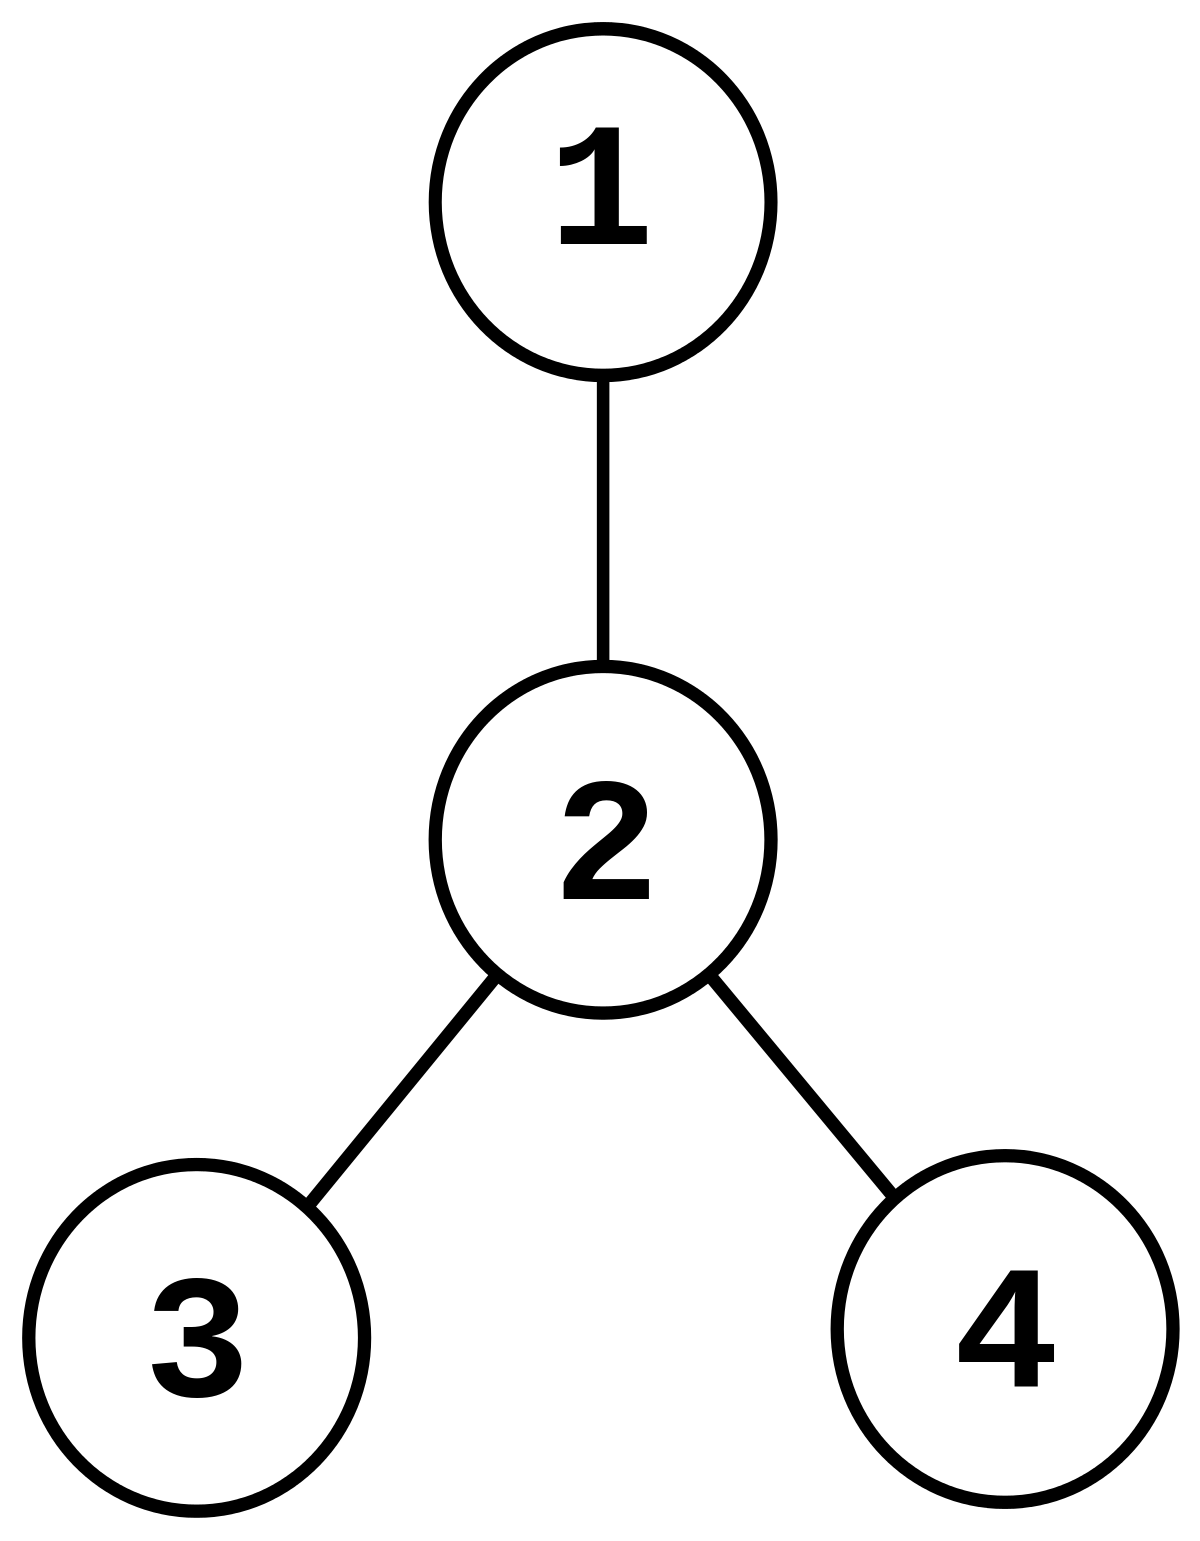
\includegraphics[width=0.3 \textwidth]{Figures/grapheNonOriente.png}
    \caption{Graphe non Orienté}
    \label{fig:Graphe non Orienté}
\end{figure}

\end{frame}
